\documentclass[tikz,border=2pt]{standalone}
\usepackage{amsmath,amssymb}
\usepackage{tikz}
\usetikzlibrary{arrows.meta}

\begin{document}
% The velocity vector gamma'(t_0) is tangent to the path, built from the derivatives of the
% coordinate functions; its length is the speed.
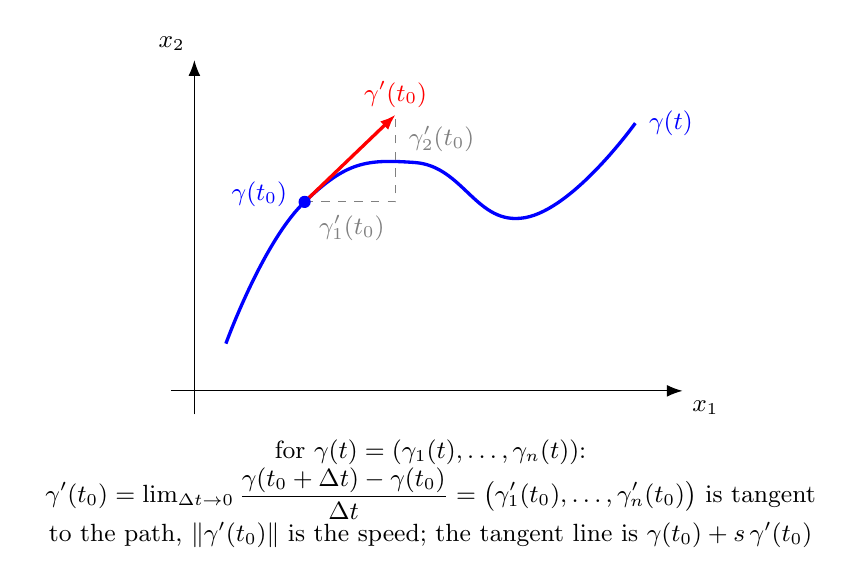
\begin{tikzpicture}[every node/.style={font=\small}, >={Latex[length=2mm]}]
	\draw[->] (-0.3,0) -- (6.2,0) node[below right] {$x_1$};
	\draw[->] (0,-0.3) -- (0,4.2) node[above left] {$x_2$};
	\draw[blue, very thick] plot[smooth, tension=0.8] coordinates {(0.4,0.6) (1.4,2.4) (2.8,2.9) (4.2,2.2) (5.6,3.4)};
	\node[blue, anchor=west, font=\small] at (5.65,3.4) {$\gamma(t)$};
	\draw[dashed, gray] (1.4,2.4) -- (2.556,2.4) -- (2.556,3.508);
	\draw[->, red, very thick] (1.4,2.4) -- (2.556,3.508) node[above, inner sep=2pt, font=\small] {$\gamma'(t_0)$};
	\fill[blue] (1.4,2.4) circle (2.2pt);
	\node[blue, anchor=east, font=\small] at (1.3,2.5) {$\gamma(t_0)$};
	\node[gray, font=\small, anchor=north] at (2.0,2.36) {$\gamma_1'(t_0)$};
	\node[gray, font=\small, anchor=west] at (2.6,3.2) {$\gamma_2'(t_0)$};
	\node[anchor=north, align=flush center, text width=10cm] at (3.0,-0.5) {for $\gamma(t)=(\gamma_1(t),\dots,\gamma_n(t))$: $\gamma'(t_0)=\lim_{\Delta t\to0}\dfrac{\gamma(t_0+\Delta t)-\gamma(t_0)}{\Delta t}=\big(\gamma_1'(t_0),\dots,\gamma_n'(t_0)\big)$ is tangent to the path, $\|\gamma'(t_0)\|$ is the speed; the tangent line is $\gamma(t_0)+s\,\gamma'(t_0)$};
\end{tikzpicture}
\end{document}
